\chapterpage{2}{Marco Teórico}
\refstepcounter{chapter} % incrementa el contador del capítulo
\addcontentsline{toc}{chapter}{Cap. 2 Marco Teórico} % opcional: que sí salga en el índice

En este capítulo se presentan los fundamentos teóricos que sustentan el diseño y desarrollo del sistema de gestión de inventario para Farmacia Selene, incluyendo los conceptos de arquitectura de sistemas, la interacción entre componentes físicos y digitales, y las tecnologías utilizadas en cada parte del proyecto.

% Se describe cómo sensores, microcontroladores, bases de datos, APIs y aplicaciones web se integran para formar una solución completa y funcional, proporcionando el soporte necesario para comprender la arquitectura general y la lógica de operación del sistema.








\section{Componentes del Sistema de Gestión de Inventario}

El sistema de gestión de inventario se diseña siguiendo una arquitectura dividida en \textbf{capas}, una práctica común en el desarrollo de sistemas de información modernos. Esta separación permite organizar mejor las funciones del sistema, facilitar su mantenimiento y permitir que cada parte evolucione de manera independiente sin afectar a las demás.

% En este proyecto, el sistema se estructura en tres capas principales: \textbf{Frontend}, \textbf{Backend} y \textbf{Capa Física}. Cada una cumple una función específica, pero todas trabajan de forma integrada para ofrecer una solución completa.

\begin{enumerate}
\item \textbf{Capa Frontend (Interfaz de Usuario):}
Es la parte del sistema con la que interactúan empleados y administradores de la farmacia. Es una aplicación web accesible desde el navegador, que muestra la información de forma clara mediante formularios, tablas, botones y gráficos.
Su función principal es permitir al usuario consultar y registrar información, como ventas, inventario o alertas. El frontend no procesa reglas complejas ni almacena datos de forma permanente; solo envía las acciones al backend y muestra las respuestas recibidas.

\item \textbf{Capa Backend (Lógica de Negocio y API):}  
El backend constituye el núcleo lógico del sistema. Es responsable de procesar la información, aplicar las reglas del negocio y gestionar el acceso a los datos almacenados en la base de datos.  
En esta capa se realizan operaciones como validar usuarios, verificar la disponibilidad de productos, calcular totales de ventas y registrar movimientos de inventario.  
La comunicación entre el frontend y el backend se realiza mediante una API (Interfaz de Programación de Aplicaciones), que define un conjunto de reglas y formatos estandarizados para el intercambio de información. Gracias a esta API, el frontend puede solicitar datos o enviar instrucciones sin conocer los detalles internos del funcionamiento del sistema.

\item \textbf{Capa Física (Sensores y Hardware):}  
Esta capa está compuesta por dispositivos físicos utilizados dentro de la farmacia, como sensores de temperatura y humedad para el control de medicamentos sensibles, así como lectores de códigos de barras para el registro de productos.  
Estos dispositivos capturan información del entorno físico y la envían automáticamente al backend, donde es almacenada y analizada. De esta manera, el sistema integra datos digitales con condiciones reales del entorno, permitiendo una supervisión más precisa y automatizada.

\end{enumerate}

La integración de estas capas permite que el sistema funcione de manera coordinada. Por ejemplo, al escanear un producto con un lector de códigos de barras (Capa Física), el backend identifica el medicamento correspondiente en la base de datos y envía la información al frontend para que sea mostrada al usuario. De forma similar, si un sensor detecta una variación anormal de temperatura, el backend puede generar una alerta que se visualiza inmediatamente en la interfaz del administrador. Esta arquitectura modular hace que el sistema sea escalable, confiable y adaptable a las necesidades futuras de la Farmacia Selene.











\secbreak
\section{Capa Frontend: Tecnologías Web}

La Capa Frontend representa la interfaz gráfica del sistema y constituye el principal medio de interacción entre los usuarios y la plataforma. Su diseño debe garantizar facilidad de uso, rapidez en la respuesta y una presentación clara de la información. 

\subsection{Tecnologías Base: HTML, CSS y JavaScript}

El desarrollo del frontend se apoya en tres tecnologías fundamentales de la web:

\begin{itemize}
\item \textbf{HTML (Lenguaje de Marcado de Hipertexto):}
Define la estructura del contenido de la aplicación. Permite organizar los elementos visibles como encabezados, formularios, tablas y contenedores donde se muestran los datos del inventario, ventas y reportes.

\item \textbf{CSS (Hojas de Estilo en Cascada):}  
Se encarga de la presentación visual del sistema. Controla aspectos como colores, tamaños, tipografía y distribución de los elementos en la pantalla, asegurando una interfaz clara, ordenada y adaptable a distintos dispositivos.

\item \textbf{JavaScript:}  
Es el lenguaje de programación que permite agregar comportamiento dinámico a la interfaz. Gracias a JavaScript, el sistema puede responder a las acciones del usuario, validar datos, actualizar información en pantalla y comunicarse con el backend sin recargar la página.

\end{itemize}

\subsection{React: Biblioteca para el Desarrollo de Interfaces}

Para facilitar la construcción de interfaces complejas y dinámicas, se utiliza \textbf{React}, una biblioteca de JavaScript ampliamente empleada en aplicaciones web modernas. React permite dividir la interfaz en \textbf{componentes}, es decir, unidades independientes que encapsulan su propia estructura y comportamiento.

Por ejemplo, el sistema puede contar con componentes específicos para la tabla de productos, el formulario de ventas o las alertas de temperatura. Esta organización mejora la legibilidad del código, facilita el mantenimiento y permite reutilizar componentes en distintas partes de la aplicación.

React también utiliza un mecanismo de actualización eficiente que modifica únicamente los elementos de la interfaz que han cambiado, lo que contribuye a un mejor rendimiento y una experiencia de usuario más fluida.

\subsection{Material-UI (MUI): Diseño y Consistencia Visual}

Para asegurar una apariencia profesional y coherente, el frontend emplea \textbf{Material-UI (MUI)}, una biblioteca de componentes prediseñados basada en el estándar de diseño Material Design.
MUI proporciona elementos visuales como botones, formularios, tablas y menús listos para usarse, lo que reduce el tiempo de desarrollo y mejora la uniformidad visual del sistema.

Entre sus principales ventajas se encuentran:

\begin{itemize}
\item \textbf{Estandarización visual:} Todos los elementos mantienen una apariencia consistente en toda la aplicación.
\item \textbf{Diseño responsivo:} La interfaz se adapta automáticamente a distintos tamaños de pantalla.
\item \textbf{Mejora de la usabilidad:} Los componentes están diseñados para ser claros, accesibles y fáciles de usar.
\end{itemize}

En conjunto, estas tecnologías permiten construir una Capa Frontend moderna, eficiente y fácil de usar, que sirve como herramienta principal para la operación diaria de la Farmacia Selene y facilita la transición de procesos manuales a un entorno digital.


\subsection{Vercel: Plataforma de Despliegue del Frontend}

Para la publicación y disponibilidad en línea de la aplicación web se utiliza \textbf{Vercel}, una plataforma de despliegue en la nube especializada en aplicaciones frontend modernas.

Vercel permite alojar aplicaciones desarrolladas con tecnologías como React de manera sencilla y automatizada. Su funcionamiento se basa en la integración con repositorios de control de versiones, lo que significa que cada vez que se actualiza el código del proyecto, la plataforma genera automáticamente una nueva versión desplegada en internet.

Entre las principales ventajas de utilizar Vercel en este proyecto se encuentran:

\begin{itemize}
    \item \textbf{Despliegue automático:} Cada actualización del sistema genera una nueva versión disponible en línea sin necesidad de configuraciones manuales complejas.
    \item \textbf{Alta disponibilidad:} La aplicación puede ser accesada desde cualquier dispositivo con conexión a internet.
    \item \textbf{Optimización de rendimiento:} Implementa técnicas de distribución global de contenido (CDN), reduciendo los tiempos de carga.
    \item \textbf{Escalabilidad:} Permite que la aplicación soporte múltiples usuarios simultáneamente sin afectar su rendimiento.
\end{itemize}

El uso de Vercel facilita que la Farmacia Selene pueda acceder al sistema desde distintos equipos dentro de la sucursal sin requerir infraestructura propia de servidores, reduciendo costos de implementación y mantenimiento.















\secbreak
\section{Capa Backend: Servidor, API y Base de Datos}

La Capa Backend es la parte interna del sistema de gestión de inventario y funciona como el centro de control de toda la información. Aunque no es visible para los usuarios, es fundamental para el correcto funcionamiento del sistema, ya que se encarga de procesar los datos, aplicar las reglas del negocio, proteger la información y coordinar la comunicación entre la interfaz de usuario, la base de datos y los dispositivos físicos.

En términos generales, el backend actúa como un intermediario inteligente: recibe las solicitudes del frontend (por ejemplo, registrar una venta o consultar el inventario), las procesa de acuerdo con las reglas establecidas y devuelve una respuesta con la información correspondiente. Para lograr esto, el backend se implementa como una \textbf{API (Interfaz de Programación de Aplicaciones)}, es decir, un conjunto de rutas y reglas que permiten el intercambio de información de forma ordenada y segura.

El desarrollo del backend se realizó utilizando el lenguaje de programación Python y herramientas modernas que facilitan la organización, el mantenimiento y la evolución del sistema.

\subsection{Python}

Python es el lenguaje de programación utilizado para desarrollar el backend del sistema. Fue elegido por su sintaxis clara y legible, lo que facilita la comprensión del código, la detección de errores y el mantenimiento del sistema, especialmente en proyectos colaborativos. Además, cuenta con un ecosistema amplio y maduro de librerías y frameworks que permiten desarrollar aplicaciones web robustas y escalables de manera eficiente.

En este sistema, Python actúa como la base sobre la cual se implementa la lógica de negocio, gestionando las operaciones de inventario, autenticación de usuarios, registro de datos de sensores y comunicación con la base de datos PostgreSQL, asegurando que el backend funcione de manera eficiente, confiable y segura.

\subsection{FastAPI: Comunicación entre el Sistema y los Usuarios}

FastAPI es el framework web utilizado para construir el backend. Un framework puede entenderse como una base de trabajo que proporciona las herramientas necesarias para recibir solicitudes, procesarlas y enviar respuestas.

FastAPI permite definir claramente qué acciones puede realizar el sistema, como consultar productos, registrar ventas o recibir datos de sensores. Cada una de estas acciones se define como un \textbf{endpoint}, que es simplemente una dirección a la que el frontend o los dispositivos pueden enviar información.

Entre las principales características de FastAPI se encuentran:

\begin{itemize}
    \item \textbf{Facilidad de uso}: Permite escribir código claro y estructurado, lo que reduce errores y facilita el mantenimiento.
    \item \textbf{Validación de datos}: Verifica automáticamente que la información recibida tenga el formato correcto antes de procesarla.
    \item \textbf{Documentación automática}: Genera una interfaz visual donde se pueden consultar y probar las funciones del sistema, lo que facilita su comprensión y verificación.
    \item \textbf{Buen rendimiento}: Está diseñado para responder de forma rápida incluso cuando el sistema recibe múltiples solicitudes al mismo tiempo.
\end{itemize}

Gracias a FastAPI, el backend puede comunicarse de manera eficiente tanto con la interfaz web como con los dispositivos físicos del sistema.

\subsection{PostgreSQL: Almacenamiento de la Información}

PostgreSQL es el sistema de base de datos utilizado para almacenar toda la información del sistema de gestión de inventario. Una base de datos puede entenderse como un repositorio organizado donde se guardan los datos de forma estructurada y segura.

Se eligió PostgreSQL debido a su confiabilidad y a su capacidad para manejar información crítica, como inventarios y registros de ventas.

La base de datos almacena información como:

\begin{itemize}
    \item Usuarios del sistema (administradores y empleados).
    \item Productos disponibles en la farmacia, incluyendo precios y existencias.
    \item Registros de ventas realizadas.
    \item Mediciones de temperatura y humedad enviadas por los sensores.
\end{itemize}

Este almacenamiento centralizado permite que la información esté siempre disponible y actualizada para todos los usuarios autorizados.

\subsection{SQLAlchemy: Manejo de la Base de Datos}

Para interactuar con la base de datos se utiliza SQLAlchemy, una herramienta que permite trabajar con los datos utilizando estructuras del propio lenguaje Python, en lugar de escribir instrucciones complejas directamente en lenguaje SQL.

Gracias a SQLAlchemy, el sistema puede:

\begin{itemize}
    \item Crear, consultar, actualizar y eliminar registros de la base de datos.
    \item Representar tablas como objetos, lo que hace el código más fácil de entender.
    \item Mantener una separación clara entre la lógica del sistema y el almacenamiento de datos.
\end{itemize}

Esto contribuye a un desarrollo más ordenado y reduce la probabilidad de errores en el manejo de la información.

\subsection{Alembic: Control de Versiones de la Base de Datos}

Durante el desarrollo del sistema se utilizó \textbf{Alembic}, una herramienta especializada en la gestión de versiones de bases de datos que trabaja en conjunto con SQLAlchemy. Su función principal es permitir la modificación estructurada y controlada del esquema de la base de datos a lo largo del tiempo.

En un proyecto en constante evolución, es común que las tablas requieran cambios, como la adición de nuevas columnas, la creación de relaciones entre entidades o la modificación de restricciones. Realizar estos cambios manualmente puede generar errores y afectar la integridad de la información. Alembic resuelve este problema mediante el uso de \textbf{migraciones}, que son archivos que describen de manera explícita las modificaciones realizadas en la estructura de la base de datos.

Entre las principales ventajas de utilizar Alembic se encuentran:

\begin{itemize}
    \item \textbf{Control de versiones del esquema:} Permite llevar un historial ordenado de los cambios estructurales en la base de datos.
    \item \textbf{Actualización controlada:} Facilita aplicar o revertir modificaciones de manera segura.
    \item \textbf{Integración con SQLAlchemy:} Detecta cambios en los modelos definidos en Python y genera scripts de migración correspondientes.
    \item \textbf{Reducción de errores:} Disminuye riesgos asociados a cambios manuales en la estructura de las tablas.
\end{itemize}

El uso de Alembic en este proyecto garantiza que la base de datos pueda evolucionar conforme crecen los requerimientos del sistema, manteniendo consistencia, trazabilidad y buenas prácticas de desarrollo.

\subsection{Railway: Plataforma de Despliegue del Backend}

Para el alojamiento y ejecución del backend en un entorno accesible desde internet se utiliza \textbf{Railway}, una plataforma de infraestructura en la nube que permite desplegar aplicaciones y bases de datos de manera sencilla.

Railway proporciona un entorno donde el servidor desarrollado con FastAPI puede ejecutarse de forma continua, permitiendo que el frontend y los dispositivos físicos se comuniquen con la API desde cualquier ubicación con conexión a internet.

Entre las principales características de Railway se encuentran:

\begin{itemize}
    \item \textbf{Despliegue simplificado:} Permite subir el proyecto directamente desde un repositorio, automatizando la configuración del servidor.
    \item \textbf{Integración con bases de datos:} Facilita la creación y administración de bases de datos PostgreSQL en la nube.
    \item \textbf{Escalabilidad automática:} Ajusta los recursos del servidor según la demanda del sistema.
    \item \textbf{Monitoreo y gestión:} Proporciona herramientas para supervisar el estado del servicio y detectar posibles errores.
\end{itemize}

Gracias a Railway, el backend del sistema permanece activo de manera constante, asegurando que las solicitudes provenientes del frontend y de los dispositivos IoT sean atendidas en tiempo real. Esto permite que el sistema funcione como una plataforma centralizada y accesible, sin necesidad de mantener servidores físicos dentro de la farmacia.
















\secbreak
\section{Capa Física: Dispositivos y Hardware}

La Capa Física corresponde al conjunto de dispositivos electrónicos que operan directamente dentro de la farmacia y que permiten vincular el sistema digital con el entorno real. Su función principal es capturar información física, como la temperatura, la humedad o los códigos de barras de los productos y enviarla al sistema informático para su procesamiento y almacenamiento.

Además de la conexión física, estos dispositivos requieren programación específica para gestionar la lectura de sensores, la comunicación con otros periféricos y el envío de datos al backend. En este proyecto, el microcontrolador ESP32 actúa como el núcleo de la capa física, siendo programado en C/C++ para coordinar todas estas funciones de manera eficiente y confiable.

Esta capa es fundamental para automatizar tareas que tradicionalmente se realizan de forma manual, reducir errores humanos y asegurar el cumplimiento de condiciones ambientales necesarias para la correcta conservación de los medicamentos. Los dispositivos que conforman esta capa se comunican con el backend mediante la red local, formando un sistema de Internet de las Cosas (IoT).

\subsection{C++}

El ESP32 se programa utilizando los lenguajes \textbf{C++}, debido a que permiten un control directo sobre el hardware y optimizan el uso de recursos del microcontrolador. Estos lenguajes son ampliamente utilizados en sistemas embebidos por su eficiencia y capacidad de manejar tareas en tiempo real, como la lectura de sensores, el control de periféricos y la comunicación con el backend del sistema.

En el proyecto de gestión de inventario de la Farmacia Selene, C++ se emplea para:

\begin{itemize}
\item Configurar y leer los sensores de temperatura y humedad (AHT10) mediante interfaces digitales como I2C.
\item Gestionar la comunicación con el lector de códigos de barras y otros periféricos conectados al ESP32.
\item Transmitir de manera confiable los datos recopilados al servidor backend usando protocolos de red como HTTP o MQTT.
\item Optimizar el uso de memoria y procesamiento del microcontrolador, asegurando un funcionamiento eficiente y estable del sistema.
\end{itemize}

Gracias al uso de C++, el microcontrolador actúa como un puente confiable entre la capa física y el sistema digital, garantizando que los datos del entorno se integren de manera efectiva en la plataforma de gestión de inventario.

\subsection{Microcontrolador ESP32-C5}

El microcontrolador \textbf{ESP32-C5} es el dispositivo central de la capa física del sistema y actúa como el \textbf{controlador principal} de la red de sensores. Su función es leer la información proveniente de los dispositivos conectados, realizar un procesamiento básico y transmitir los datos al servidor backend a través de la red inalámbrica.

El ESP32-C5 es una variante de la familia ESP32 diseñada específicamente para aplicaciones de Internet de las Cosas (IoT), destacando por integrar conectividad \textbf{Wi-Fi 6 (802.11ax)} y Bluetooth Low Energy (BLE) en un solo chip. La incorporación de Wi-Fi 6 permite una comunicación más eficiente, menor latencia y mejor desempeño en entornos con múltiples dispositivos conectados, como es el caso de una farmacia con sistemas digitales concurrentes.

En el contexto del sistema propuesto, el ESP32-C5 funciona como un intermediario entre el entorno físico y el sistema de gestión digital, permitiendo la digitalización de variables ambientales críticas para el almacenamiento de medicamentos.

Entre sus principales funciones dentro del sistema se encuentran:
\begin{itemize}
    \item Leer periódicamente los valores de temperatura y humedad del entorno mediante sensores conectados.
    \item Gestionar la comunicación con sensores y periféricos a través de interfaces como I2C, SPI y GPIO.
    \item Procesar los datos de manera preliminar antes de su envío.
    \item Enviar los datos recopilados al backend para su almacenamiento, monitoreo y análisis.
    \item Mantener una conexión estable con la red Wi-Fi de la farmacia utilizando el estándar Wi-Fi 6.
\end{itemize}

El uso del ESP32-C5 permite que la captura de datos ambientales sea automática y continua, sin necesidad de intervención humana, lo que incrementa la confiabilidad del monitoreo y facilita la supervisión en tiempo real. Además, su bajo consumo energético y su capacidad de operación en redes densas lo convierten en una solución adecuada para sistemas IoT en entornos comerciales.

\begin{figure}[H]
    \centering
    \fbox{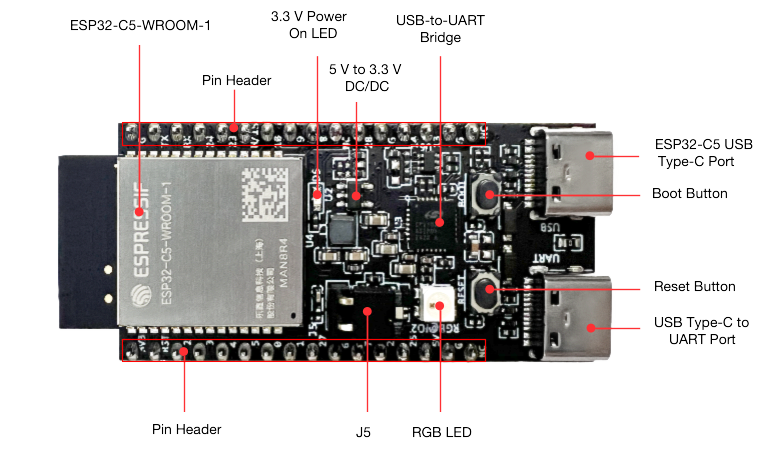
\includegraphics[width=0.7\textwidth]{0_imagenes/Cap2MarcoTeorico/ESP32-C5-DevKitC-1_v1.1_callouts.png}}
    \caption{Microcontrolador ESP32-C5}
    \label{fig:mi_imagen}
    
    \vspace{0.2cm}
    \footnotesize \textbf{Fuente:} \url{https://docs.espressif.com/projects/esp-dev-kits/en/latest/esp32c5/_images/ESP32-C5-DevKitC-1_v1.1_callouts.png}
\end{figure}


\subsection{Sensor de Temperatura y Humedad AHT10}

Para el monitoreo ambiental se utiliza el \textbf{sensor digital de temperatura y humedad AHT10}, el cual permite medir de forma continua las condiciones del entorno donde se almacenan los medicamentos. Este sensor proporciona lecturas confiables y estables, ya que viene calibrado de fábrica y ha sido diseñado específicamente para aplicaciones de control ambiental y sistemas IoT de bajo consumo.

El AHT10 se comunica con el microcontrolador mediante la interfaz \textbf{I²C}, lo que facilita su integración con el ESP32-C5 y permite la conexión de múltiples sensores en un mismo bus de comunicación. Esta característica resulta especialmente útil en entornos donde se requiere monitorear varias áreas de almacenamiento de manera simultánea.

Dentro del sistema, el sensor AHT10 cumple las siguientes funciones:

\begin{itemize}
    \item Medir la \textbf{temperatura} del área de almacenamiento de medicamentos con precisión de ±0.3 °C.
    \item Medir la \textbf{humedad relativa} del ambiente con precisión de ±2\%.
    \item Transmitir las mediciones al microcontrolador ESP32-C5 mediante la interfaz I²C.
    \item Permitir la generación de alertas tempranas en caso de que las condiciones ambientales superen los rangos recomendados para los medicamentos.
\end{itemize}

La información obtenida por el sensor AHT10 es fundamental para el control de medicamentos sensibles a la temperatura y la humedad. Gracias al monitoreo continuo, el sistema puede detectar condiciones fuera de los rangos recomendados y notificar al personal de la farmacia para que tome las acciones necesarias de manera oportuna.

De esta forma, el sistema contribuye al cumplimiento de buenas prácticas de almacenamiento y ayuda a preservar la calidad y seguridad de los productos farmacéuticos, integrando de manera eficiente la capa física de sensores con la capa de procesamiento y comunicación del ESP32-C5.


\begin{figure}[H]
    \centering
    \fbox{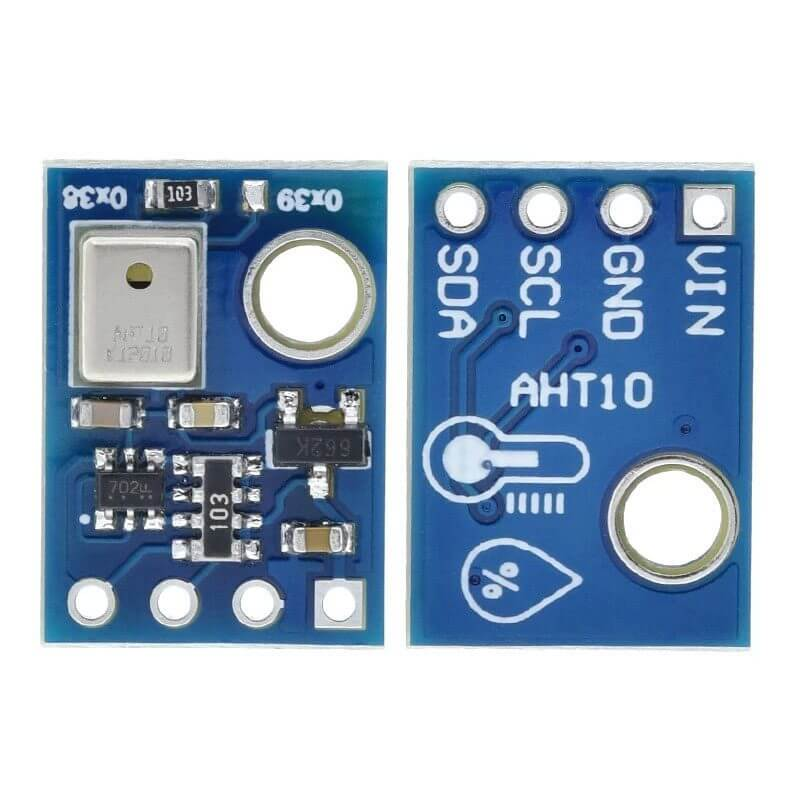
\includegraphics[width=0.4\textwidth]{0_imagenes/Cap2MarcoTeorico/AR3107-AHT10-Sensor-de-Temperatura-y-Humedad-V2-800x800.jpg}}
    \caption{Sensor AHT10}
    \label{fig:mi_imagen}
    
    \vspace{0.2cm}
    \footnotesize \textbf{Fuente:} \url{https://uelectronics.com/wp-content/uploads/2022/04/AR3107-AHT10-Sensor-de-Temperatura-y-Humedad-V2-800x800.jpg}
\end{figure}

\subsection{Lector de Códigos de Barras}

El lector de códigos de barras es un dispositivo de entrada que permite registrar productos de manera rápida y precisa. Su objetivo principal es reemplazar la captura manual de códigos, reduciendo errores y agilizando los procesos de venta y control de inventario.

Cuando un empleado escanea un producto, el lector obtiene el código correspondiente y lo envía automáticamente al sistema. Este código es utilizado por la aplicación para identificar el medicamento dentro de la base de datos.

Una vez leído el código, la aplicación web solicita al backend la información asociada al producto, como su nombre, precio y cantidad disponible. Esta información se muestra al usuario de forma automática, haciendo el proceso más rápido y eficiente.












\secbreak
\section{Herramientas de Desarrollo}

Además de las tecnologías que conforman directamente la arquitectura del sistema (frontend, backend y capa física), el desarrollo del proyecto requirió el uso de herramientas especializadas que permitieron organizar el código, mantener un control estructurado de los cambios y facilitar el proceso de programación.

Estas herramientas no forman parte del sistema final utilizado por la Farmacia Selene, pero son fundamentales durante la etapa de desarrollo, ya que garantizan orden, trazabilidad y buenas prácticas de ingeniería de software.

\subsection{Git y GitHub: Control de Versiones y Gestión del Código}

Para mantener un desarrollo organizado y estructurado del sistema se utilizaron herramientas de control de versiones, las cuales permiten registrar y administrar los cambios realizados en el código fuente a lo largo del proyecto.

\begin{itemize}
    \item \textbf{Git:} Sistema de control de versiones distribuido que permite llevar un historial de modificaciones del código, facilitando la recuperación de versiones anteriores y la identificación de cambios realizados.
    
    \item \textbf{GitHub:} Plataforma en línea que permite alojar repositorios Git y almacenar el código fuente del proyecto de manera centralizada, conservando el registro completo de su evolución.
\end{itemize}

El uso conjunto de estas herramientas permitió garantizar la trazabilidad del desarrollo y mantener una documentación técnica clara de las distintas etapas del proyecto.

\subsection{Entornos de Desarrollo Integrados (IDE)}

Un Entorno de Desarrollo Integrado (IDE) es una aplicación de software que proporciona herramientas especializadas para escribir, organizar y depurar código de manera eficiente. Estas herramientas suelen incluir editor de texto avanzado, resaltado de sintaxis, autocompletado, detección de errores y gestión estructurada de proyectos.

Durante el desarrollo del sistema se utilizaron distintos IDE según el componente trabajado:

\begin{itemize}
    \item \textbf{PyCharm:} Utilizado principalmente para el desarrollo del backend en Python y la implementación de la lógica del sistema.
    \item \textbf{Visual Studio Code (VS Code):} Empleado en el desarrollo del frontend con tecnologías web como HTML, CSS, JavaScript y React.
    \item \textbf{DataGrip:} Utilizado para la administración y consulta de la base de datos PostgreSQL, facilitando la visualización y manipulación estructurada de los datos.
\end{itemize}

El uso de estos entornos de desarrollo permitió mejorar la organización del proyecto, optimizar la detección temprana de errores y mantener una estructura clara en cada una de las capas del sistema. Esto contribuyó a un proceso de desarrollo más eficiente y ordenado.

\subsection{JSON: Formato de Intercambio de Datos}

JSON (JavaScript Object Notation) es un formato ligero de intercambio de datos ampliamente utilizado en aplicaciones web modernas. Su estructura se basa en pares de clave y valor, lo que permite representar información de manera organizada y fácilmente interpretable tanto por humanos como por sistemas informáticos.

Una de las principales ventajas de JSON es su simplicidad y compatibilidad con múltiples lenguajes de programación, lo que lo convierte en un estándar común para la comunicación entre aplicaciones. En arquitecturas basadas en APIs, como la utilizada en este proyecto, JSON se emplea para enviar y recibir información entre el frontend, el backend y otros sistemas externos.

En el sistema de gestión de inventario desarrollado para la Farmacia Selene, JSON se utiliza como formato principal para transmitir información entre la aplicación web y el servidor backend. Por ejemplo, cuando el frontend solicita la información de un producto, la API responde con una estructura JSON que contiene los datos correspondientes, los cuales son procesados y mostrados en la interfaz del usuario.

El uso de JSON facilita la validación de datos, mejora la interoperabilidad entre sistemas y permite manejar información de forma estructurada dentro de la arquitectura del sistema.

\subsection{JSON Web Token (JWT): Autenticación y Seguridad}

JSON Web Token (JWT) es un estándar abierto utilizado para transmitir información de forma segura entre diferentes partes de un sistema. Este mecanismo se utiliza principalmente para la autenticación de usuarios en aplicaciones web y servicios basados en APIs.

Un token JWT consiste en una cadena de texto firmada digitalmente que contiene información codificada sobre el usuario y su sesión. Cuando un usuario inicia sesión en el sistema, el servidor genera un token que se envía al cliente. Posteriormente, este token se incluye en cada solicitud realizada a la API para verificar la identidad del usuario.

El uso de JWT ofrece diversas ventajas en sistemas distribuidos, entre las que destacan:

\begin{itemize}
\item Permite autenticar usuarios sin mantener sesiones activas en el servidor.
\item Reduce la carga del sistema al evitar consultas constantes a la base de datos para validar sesiones.
\item Facilita la comunicación segura entre aplicaciones web y servicios backend.
\end{itemize}

En el sistema desarrollado para la Farmacia Selene, JWT se utiliza para controlar el acceso a las diferentes funciones de la API. De esta manera, únicamente los usuarios autenticados pueden consultar información del inventario, registrar ventas o modificar datos dentro del sistema.












